\let\lesson\undefined
\newcommand{\lesson}{\phantomlesson{Bài 16.}}
\setcounter{section}{2}
\section{Trắc nghiệm nhiều phương án lựa chọn}
\setcounter{ex}{0}
\Opensolutionfile{ans}[ans/VN10-2022-PH-TP025-TN]
% ===================================================================
\begin{ex}\mkstar{1}
	$\si{\kilo\watt\cdot\hour}$ là đơn vị của
	\choice
	{\True công}
	{công suất}
	{hiệu suất}
	{lực}
	\loigiai{}
\end{ex}
% ===================================================================
\begin{ex}\mkstar{1}
	Đơn vị nào sau đây \textbf{không} được dùng làm đơn vị đo công suất?
	\choice
	{$\si{\watt}$}
	{\True $\si{\joule\cdot\second}$}
	{$\si{HP}$}
	{$\si{\kilogram\cdot\meter^2/s^3}$}
	\loigiai{}
\end{ex}
% ===================================================================
\begin{ex}\mkstar{1}
	Công suất được xác định bằng
	\choice
	{giá trị công thực hiện được}
	{tích của công và thời gian thực hiện công}
	{công thực hiện được trên một đơn vị chiều dài}
	{\True công thực hiện được trong một đơn vị thời gian}
	\loigiai{}
\end{ex}
% ===================================================================
\begin{ex}\mkstar{1}
Đơn vị nào sau đây \textbf{không} phải là đơn vị của công suất?	
	\choice
	{Oát (W)}
	{Jun/giây (J/s)}
	{Mã lực (HP)}
	{\True Jun (J)}
	\loigiai{}
\end{ex}
% ===================================================================
\begin{ex}\mkstar{1}
	$\SI{1}{\watt}$ bằng
	\choice
	{$\SI{1}{\joule\cdot\second}$}
	{\True $\SI{1}{\joule/\second}$}
	{$\SI{10}{\joule\cdot\second}$}
	{$\SI{10}{\joule/\second}$}
	\loigiai{}
\end{ex}
% ===================================================================
\begin{ex}\mkstar{2}
	Một bóng đèn sợi đốt có công suất $\SI{100}{\watt}$ tiêu thụ năng lượng $\SI{1000}{\joule}$. Thời gian thắp sáng bóng đèn là
	\choice
	{$\SI{1}{\second}$}
	{\True $\SI{10}{\second}$}
	{$\SI{100}{\second}$}
	{$\SI{1000}{\second}$}
	\loigiai{}
\end{ex}
% ===================================================================
\begin{ex}\mkstar{2}
		Một động cơ điện cung cấp công suất $\SI{15}{kW}$ cho một cần cẩu nâng vật có khối lượng 1 tấn lên cao $\SI{15}{m}$. Thời gian tối thiểu để thực hiện công việc này bằng bao nhiêu? Lấy $g=\SI{10}{m/s^2}$.
	\choice
	{$\SI{12}{s}$}
	{\True $\SI{10}{s}$}
	{$\SI{14}{s}$}
	{$\SI{18}{s}$}
	\loigiai{Áp dụng công thức tính công suất:
		$$\calP = \dfrac{A}{t} \Rightarrow t = \dfrac{A}{\calP}  = \dfrac{mgs}{\calP} = \SI{10}{s}.$$}
\end{ex}
% ===================================================================
\begin{ex}\mkstar{2}
	Phát biểu nào sau đây là đúng?
	\choice
	{Máy có công suất lớn thì hiệu suất của máy đó nhất định cao}
	{Hiệu suất của một máy có thể lớn hơn 1}
	{Máy có hiệu suất cao thì công suất của máy nhất định lớn}
	{\True Máy có công suất lớn thì thời gian sinh công sẽ nhanh}
	\loigiai{Công suất là đại lượng đo bằng công sinh ra trong một đơn vị thời gian. Do đó máy có công suất lớn thì thời gian sinh công sẽ nhanh.}
\end{ex}
% ===================================================================
\begin{ex}\mkstar{2}
	Một vật khối lượng $\SI{1500}{kg}$ được cần cẩu nâng đều lên độ cao $\SI{20}{m}$ trong khoảng thời gian $\SI{15}{s}$. Lấy $g = \SI{10}{m/s}^2$. Công suất trung bình của lực nâng của cần cẩu là
	\choice
	{$\SI{15000}{W}$}
	{$\SI{22500}{W}$}
	{\True $\SI{20000}{W}$}
	{$\SI{1000}{W}$}
	\loigiai{	Do nâng đều nên $F = P = mg$.
		
		Công suất trung bình của lực nâng
		
		$$\calP = \dfrac{A}{t} = \dfrac{mgh}{t} = \SI{20000}{W}.$$}
\end{ex}
\Closesolutionfile{ans}
\section{Trắc nghiệm đúng/sai}
\setcounter{ex}{0}
\Opensolutionfile{ans}[ans/VN10-2022-PH-TP025-TF]
% ===================================================================
\begin{ex}\mkstar{2}
	Cần cẩu nâng một container nặng 2 tấn theo phương thẳng đứng từ vị trí nằm yên với gia tốc không đổi. Sau $\SI{5}{\second}$ container đạt vận tốc $\SI{10}{\meter/\second}$. Bỏ qua mọi lực cản. Lấy $g=\SI{10}{\meter/\second^2}$.
	\choiceTF[t]
	{\True Gia tốc của container là $\SI{2}{\meter/\second^2}$}
	{Công của lực nâng thực hiện được trong $\SI{5}{\second}$ đầu tiên là $\SI{600}{\joule}$}
	{\True Công suất trung bình lực nâng của cần cẩu trong thời gian $\SI{5}{\second}$ là $\SI{120}{\kilo\watt}$}
	{Công suất tức thời của cần cẩu tại $t=\SI{5}{\second}$ là $\SI{2400}{\watt}$}
	\loigiai{
	\begin{enumerate}[label=\alph*)]
		\item Đúng.
		\item Sai. Lực nâng của cần cẩu:
		$$F=m\left(g+a\right)=\SI{24}{\newton}.$$
		\item Đúng.
		\item Sai. Công suất tức thời: $$\calP_t=F\cdot v_t=F\cdot at=24000\cdot2\cdot5=\SI{240}{\kilo\watt}.$$
	\end{enumerate}
	}
\end{ex}
% ===================================================================
\begin{ex}\mkstar{3}
	Một ô tô có khối lượng 1 tấn và công suất của động cơ là $\SI{5}{\kilo\watt}$. Giai đoạn đầu, ô tô chuyển động thẳng đều trên mặt đường nằm ngang với tốc độ $\SI{36}{\kilo\meter/\hour}$. Giai đoạn sau, ô tô tăng tốc chuyển động nhanh dần đều và sau khi đi thêm được $\SI{125}{\meter}$ thì đạt tốc độ $\SI{54}{\kilo\meter/\hour}$. Biết độ lớn lực ma sát không đổi trong suốt quá trình ô tô chuyển động.
	\choiceTF[t]
	{\True Giai đoạn đầu, lực ma sát của mặt đường tác dụng lên ô tô là $\SI{500}{\newton}$}
	{\True Gia tốc của ô tô trong giai đoạn chuyển động nhanh dần đều là $\SI{0.5}{\meter/\second^2}$}
	{\True Khi ô tô chuyển động nhanh dần đều thì lực kéo của động cơ bằng $\SI{1000}{\newton}$}
	{\True Giai đoạn sau, công suất trung bình của động cơ ô tô sau khi đi thêm $\SI{125}{\meter}$ là $\SI{12.5}{\kilo\watt}$}
	\loigiai{}
\end{ex}
\Closesolutionfile{ans}
\section{Tự luận}
\setcounter{ex}{0}
\Opensolutionfile{ans}[ans/VN10-2022-PH-TP025-TL]

% ======================================================================
\begin{ex}\mkstar{2}
	Một vật có khối lượng 1,5 tấn được cần cẩu nâng đều lên độ cao $\SI{20}{m}$ trong khoảng thời gian $\SI{20}{s}$. Lấy $g=\SI{10}{m/s^2}$. Tính công suất trung bình của lực nâng của cần cẩu.
	\loigiai{Lực kéo của cần cẩu để nâng vật đi lên thẳng đều:
		$$F=P=mg=\SI{15000}{N}.$$
		
		Vận tốc nâng:
		$$v=\dfrac{s}{t} = \SI{1}{m/s}.$$
		
		Công suất trung bình của lực nâng của cần cẩu:
		$$\calP = Fv = \SI{15000}{W}.$$}
\end{ex}

% ======================================================================
\begin{ex}\mkstar{2}
Coi công suất trung bình của trái tim là $\SI{3}{W}$. Nếu một người sống 70 tuổi thì công của trái tim thực hiện là bao nhiêu? Một ô tô tải muốn thực hiện được công này phải thực hiện trong thời gian bao lâu? Coi công suất ô tô tải là $\xsi{3\cdot 10^5}{W}$.	
	\loigiai{Đổi 70 năm bằng 25550 ngày.
		
		Một người sống 70 tuổi thì công của trái tim thực hiện được:
		
		$$A_2 = P_2t_2 = \SI{6622560000}{J}.$$
		
		Một ô tô tải muốn thực hiện công này phải thực hiện trong thời gian:
		
		$$t_3 = \dfrac{A_2}{P_3} = \SI{22075,2}{s} = \SI{6,132}{h}.$$}
\end{ex}
% ======================================================================
\begin{ex}\mkstar{2}
	Một gàu nước có khối lượng 10 kg được kéo cho chuyển động thẳng đều lên độ cao 5 m trong khoảng thời gian 1 phút 40 s. Tính công suất trung bình của lực kéo. Lấy $g=10\ \text{m/s}^2$.
	\loigiai{Thời gian $t=1\ \text{phút}\ 40\ \text{s} = 1\cdot\SI{60}{\second} +\SI{40}{\second}= \SI{100}{\second}$.
		
		Gàu nước chuyển động thẳng đều nên lực kéo có chiều hướng lên trên và có độ lớn đúng bằng trọng lực 
		\begin{align*}
			F=P=mg.
		\end{align*}
		Công để kéo gàu nước thẳng đều: 
		\begin{equation*}
			A=Fh=mgh.
		\end{equation*}
		Công suất trung bình của lực kéo:
		\begin{equation*}
			\calP=\dfrac{A}{t} =\dfrac{mgh}{t}=\dfrac{\SI{10}{\kilogram}\cdot\SI{10}{\meter/\second^2}\cdot\SI{5}{\meter}}{\SI{100}{\second}} =\SI{5}{\watt}.
	\end{equation*}}
\end{ex}
% ======================================================================
\begin{ex}\mkstar{2}
		Động cơ của một thang máy tác dụng lực kéo $\SI{20000}{N}$ để thang máy chuyển động thẳng lên trên trong $\SI{10}{s}$ và quãng đường đi được tương ứng là $\SI{18}{m}$. Công suất trung bình của động cơ là bao nhiêu?
	\loigiai{Công suất trung bình của động cơ:
				$$\calP = \dfrac{A}{t} = \dfrac{Fs}{t} = \SI{36000}{W}  = \SI{36}{kW}.$$}
\end{ex}
% ======================================================================
\begin{ex}\mkstar{2}
	Kỉ lục trong leo cầu thang được xác lập vào ngày 4/2/2003. Theo đó một vận động viên đã leo 86 tầng với 1576 bậc cầu thang trong 9 phút 33 giây. Mỗi bậc cầu thang cao $\SI{20}{\centi\meter}$ và vận động viên nặng $\SI{70}{\kilogram}$. Tính công suất trung bình của vận động viên này.
	\loigiai{
	Quãng đường đi: $s=1576\cdot0,2=\SI{315.2}{\meter}$.\\
	Công suất trung bình của vận động viên:
	$$\calP=\dfrac{A}{t}=\dfrac{mgs}{t}\approx\SI{377.4}{\watt}.$$
	}
\end{ex}
% ======================================================================
\begin{ex}\mkstar{2}
	Trong mùa sinh sản, cá hồi bơi dọc theo con sông dài $\SI{3000}{\kilo\meter}$ trong 90 ngày để đến thượng nguồn của con sông. Trong suốt quá trình này, trung bình mỗi con cá hồi phải sinh công $\SI{1.7E6}{\joule}$.
	\begin{enumerate}[label=\alph*)]
		\item Tính công suất trung bình của cá hồi.
		\item Tính lực trung bình của cá hồi khi bơi.
	\end{enumerate}
	\loigiai{
	\begin{enumerate}[label=\alph*)]
		\item $\SI{90}{\text{ngày}}=90\cdot86400=\SI{7776000}{\second}$.\\
		Công suất trung bình của cá hồi: $\calP=\dfrac{A}{t}=\dfrac{\SI{1.7E6}{}}{7776000}\approx\SI{0.22}{\joule}$.
		\item Tốc độ trung bình của cá hồi: $v=\dfrac{s}{t}\approx\SI{0.39}{\meter/\second}$.\\
		Lực trung bình của cá hồi khi bơi: $F=\dfrac{\calP}{v}\approx\SI{0.56}{\newton}$.
	\end{enumerate}
	}
\end{ex}
% ======================================================================
\begin{ex}\mkstar{2}
	Động cơ của máy bay Airbus A320 có công suất $\SI{384}{HP}$. Để cất cánh tốt nhất, máy bay cần đạt tốc độ $\SI{308}{\kilo\meter/\hour}$. Khi bay ở độ cao ổn định, tốc độ trung bình của máy bay là $\SI{1005}{\kilo\meter/\hour}$ và để tiết kiệm nhiên liệu thì tốc độ trung bình là $\SI{968}{\kilo\meter/\hour}$. Tính lực kéo máy bay trong từng trường hợp trên. Biết $\SI{1}{HP} \approx \SI{746}{\watt}$.
	\loigiai{
	Công suất động cơ $\calP=384\cdot746=\SI{286464}{\watt}$.\\
	Lực kéo của động cơ máy bay trong từng trường hợp:
	\begin{itemize}
		\item Ở tốc độ $\SI{308}{\kilo\meter/\hour}$ ($v_1\approx\SI{85.6}{\meter/\second}$): $F_1=\dfrac{\calP}{v_1}\approx\SI{3346.5}{\newton}$.
		\item Ở tốc độ $\SI{1005}{\kilo\meter/\hour}$ ($v_2\approx\SI{279.2}{\meter/\second}$): $F_2=\dfrac{\calP}{v_2}\approx\SI{1026}{\newton}$.
		\item Ở tốc độ $\SI{968}{\kilo\meter/\hour}$ ($v_3\approx\SI{268.9}{\meter/\second}$): $F_3=\dfrac{\calP}{v_3}\approx\SI{1065.3}{\newton}$.
	\end{itemize}
	}
\end{ex}
% ======================================================================
\begin{ex}\mkstar{4}
	Một ô tô khối lượng 1 tấn đang hoạt động với công suất $\SI{5}{kW}$ và chuyển động thẳng đều với vận tốc $\SI{54}{km/h}$ thì lên dốc. Hỏi động cơ ô tô phải hoạt động với công suất bằng bao nhiêu để có thể lên dốc với tốc độ như cũ? Biết hệ số ma sát giữa bánh xe và mặt đường không đổi, dốc nghiêng góc $\SI{2,3}{^\circ}$ so với mặt đường nằm ngang và $g = \SI{10}{m/s}^2.$	
	\loigiai{Đổi 1 tấn $= \SI{1000}{kg}; \SI{5}{kW} = \SI{5000}{W}; \SI{54}{km/h} = \SI{15}{m/s}.$
		
		Khi xe ô tô chuyển động thẳng đều: 
		
		$$F'_\text{ms} = F'_\text{k} = \dfrac{\calP'}{v} = \xsi{\dfrac{1000}{3}}{\newton}.$$
		
		Hệ số ma sát là:
		
		$$\mu = \dfrac{F'_\text{ms}}{mg} = \dfrac{1}{30}.$$
		
		Khi ô tô chuyển động lên dốc, các lực tác dụng lên ô tô được biểu diễn 
		
		
		\begin{center}
			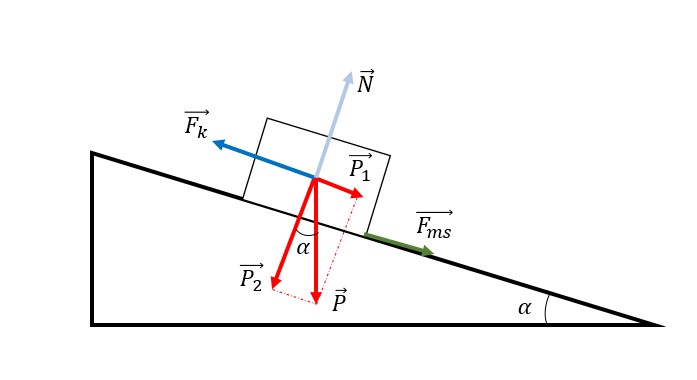
\includegraphics[scale=0.8]{../figs/VN10-2022-PH-TP027-1.jpg}
		\end{center}
		Khi lực kéo ô tô khi lên dốc có giá trị:
		$$F_\text{k} = F_\text{ms} + P_1 = \mu mg \cos \alpha + mg\sin \alpha = \SI{734,38}{N}.$$
		Để có thể lên dốc với tốc độ như cũ, ô tô phải hoạt động với công suất:
		$$\calP = F_\text{k} v = \SI{11015,7}{W}.$$}
\end{ex}

\Closesolutionfile{ans}
